\section{Conclusion and Future Work}

% The goal of this paper was to provide a clear understanding of deep neural network for document image classification. The scop
% This work presents a document classifier based on deep convolutional neural network.
% To overcome the small size of the dataset, we initialize the network with the model trained on ImageNet.
% The experimental results show that the proposed approach significantly outperforms previous work both based on either heuristics and learning based approaches.
% Being the initial and an important step of the document image processing pipeline, the significant improvement will help improving the overall performance of the later steps.
% This work may lead to further interesting research for the \ac{dip} for other classification tasks with less amount of data.


%In document image classification, the earlier works report a significant improvement when transfer learning is used. The features from a deep \ac{cnn} are adopted that was trained on a huge number of images. However, the effect of training on a huge number of documents   and then using those features for classification remained unexplored. Furthermore, there is no study of very deep \ac{cnn}s for document image classification. Therefore, it is necessary to perform a thorough evaluation of the above-mentioned gaps. 
%The presented approach explores the impact of the deep \ac{cnn} architectures and ampunt of training data.
The outcome of the study brings insights both for the deep neural network architectures and the amount of required training data. The proposed approach of training on document images and then finetuning for a document based dataset improved the error by $60\,\%$.
We show that the random initialization performs worst and initialization based on document images performs best.
Furthermore, on the large-scale RVL-CDIP dataset, VGG-16 outperforms the other networks.
Finally, a relative error reduction of $11.5\,\%$ compared to the \sota is achieved. 
Future work may evaluate recurrent neural networks or a combination of convolutional and recurrent neural networks to improve the performance further.


%\vspace{-0.5cm}
% \section*{Acknowledgment}
% We are highly thankful to Dr. David Doermann for providing us the dataset Tobacco-3482 for the experiments. This work was partially funded by the BMBF project Kallimachos (01UG1415C).
% In visual saliency estimation, many researchers have no-
% ticed that it is often insufficient to use only one metric in
% model comparison. Usually, only marginal improvements
% can be achieved with some metrics, while the scores given
% by certain metrics can be easily improved to a large exten-
% t by using simple tricks (
% e.g.
% , re-parameterizations, Gaus-
% sian smoothing, center-biased re-weighting and border cut).
% This makes the selection of evaluation metric a much con-
% fusing step in developing new saliency models. Therefore,
% it is necessary to address a long-standing concern: how to
% measure the performance (in other words, the reliability) of
% a metric in evaluating saliency maps and saliency models?
% To compare various metrics, we conduct extensive sub-
% jective tests to find how saliency maps are assessed by sub-
% jects.  By assuming that human performs the best in as-
% sessing saliency maps, we can thus provide a quantitative
% performance score for each metric. Among nine represen-
% tative metrics, we find that
% NSS
% performs the most consis-
% tently with the human-being, while the classic
% AUC
% only

% ranks the
% 4
% th
% place with the prediction accuracy of
% 78
% .
% 0%
% .
% That also explains the reason why human often thinks ex-
% isting models are far from perfect in real-world application-
% s, even though some models can achieve extremely high
% AUC
% scores. Moreover, shuffled metrics such as
% sAUC
% and
% rAUC
% , which are frequently used in recent studies, perform
% inconsistent with subjects. This is due to the fact that shuf-
% fled metrics are designed to alleviate the center-bias effect.
% However, it is often insufficient to focus only on the cen-
% ter regions. For instance, a distractor wrongly popped-out
% at the corner of ESM will be ignored in computing
% sAUC
% ,
% since shuffled fixations distribute around image center as
% well. Therefore, the feasibility of using shuffled fixations in
% the evaluation should be carefully instigated.
% In this study, we propose a data-driven metric for com-
% prehensive evaluation of saliency models. This metric dif-
% fers from existing metrics in two aspects: First, it is learned
% from user-data other than being heuristically designed. Sec-
% ond, it focuses on predicting the ordering of ESMs other
% than assigning each ESM a real-valued score. Experimental
% results show that this CNN-based metric outperforms nine
% representative metrics in assessing saliency maps. We al-
% so provide three ranking lists of 23 models to reveal the
% best saliency models. In the future work, we will incorpo-
% rate eye-tracking devices so as to discover the latent mech-
% anisms in assessing saliency maps. We will also explore
% the feasibility of designing new saliency models under the
% guidance of such a CNN-based metric.


\begin{figure}
        \centering
        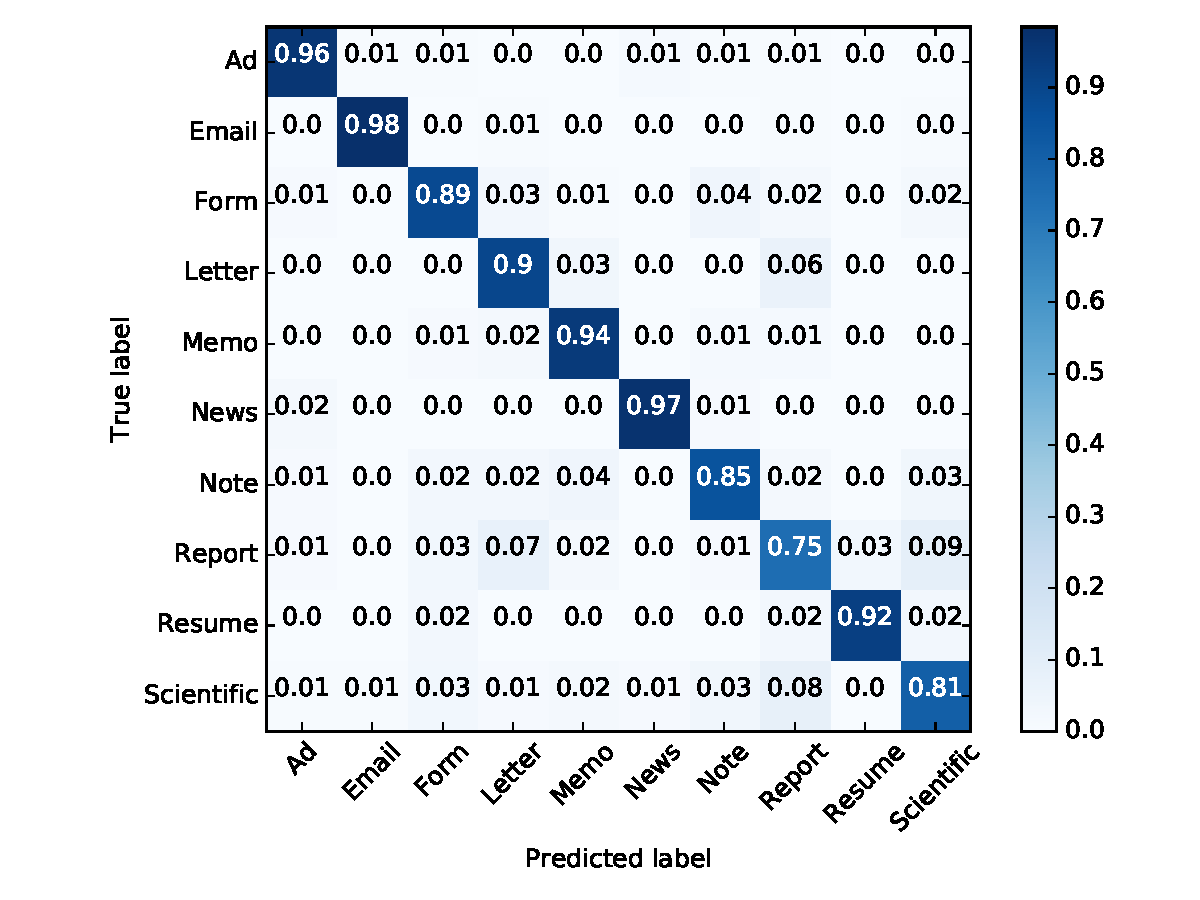
\includegraphics[width=\linewidth]{confusion_vgg.pdf}
        \caption{Confusion Matrix by a VGG-16 network trained on the Tobacco-3482 dataset.}
\label{fig:confusion}
\end{figure}
